\documentclass[12pt,letterpaper]{article}
\usepackage{amsmath,amsthm,amsfonts,amssymb,amscd}
\usepackage{fullpage}
\usepackage{lastpage}
\usepackage{enumerate}
\usepackage{fancyhdr}
\usepackage{tikz}
\usetikzlibrary{arrows, automata}
\usepackage{mathrsfs}
\usepackage{dsfont}
\usepackage[margin=3cm]{geometry}
\setlength{\parindent}{0.0in}
\setlength{\parskip}{0.05in}
\usepackage{caption}
\usepackage{subcaption}
\usepackage{float}

\newcommand\refobj{\textmd{ref}}
\newcommand\prob{\mathbb{P}}
\newcommand\E{\mathbb{E}}
\DeclareMathOperator*{\argmin}{\arg\!\min}

\begin{document}
\section*{Introduction}
Let $\Gamma$ represent the knowledge of the table. $\Gamma$ is composed of $\gamma_1, \ldots, \gamma_n$, corresponding to the objects on the table, and $\gamma_{\textmd{wall}_1}, \gamma_{\textmd{wall}_2}, \gamma_{\textmd{wall}_3}, \gamma_{\textmd{wall}_4}$, corresponding to the four walls (edges) of the table. Each $\gamma$ contains position and dimension information about the object in question.   \\
\\
Let $\lambda$ be the command the user gives, consisting of a distance $\lambda_d$ a direction (relation) $\lambda_r$ and a reference object $\lambda_f$. For the sake of testing this algorithm, we will assume perfect ability to parse the command and extract this information. Therefore we assume there is a perfect correspondence between $\lambda_f$ and $\gamma_\refobj$, where $\gamma_\refobj \in \{\gamma_1, \ldots, \gamma_n\}$. In addition, we assume that the direction is in the set $\{$left, right, in front, behind$\}$ and map $\lambda_r$ to the corresponding direction vectors $\{[1, 0], [-1, 0], [0, 1], [0, -1]\}$.  Underlying this assumption is the larger assumption that all commands map to a single direction vector - discussion of how we plan to improve this can be found later in this paper. We assume that the distance $\lambda_d$ of a command is independent of the direction $\lambda_r$. Finally, we only deal with two dimensions, so don't consider commands that involve the $z$-axis. \\
\\
As an example, if the command is `five inches to the right of the bowl', then we have $\lambda_d = 5$, $\lambda_r = [1, 0]$, $\lambda_f = $ the bowl. \\
\\
Our goal then is to estimate a function $\mathbb{P}(x, y | \lambda, \Gamma)$ which gives the probability that a user was referring to the point $(x, y)$ given the command $\lambda$ and world $\Gamma$. \\
\\
From the command and reference, we calculate a naive mean, which is the point you would select if you went exactly the distance specified by the command, in the direction specified by the command. From this we calculate four features for a log-linear model. 

\section*{Feature Calculation}
\subsection*{Calculating $\hat{\mu}$}
The naive mean, $\hat{\mu}$, is what is obtained by going exactly the distance specified in the command from the edge of the object. This is calculated as follows:
\[
\hat{\mu} = \begin{cases} 
\gamma_\refobj.center + \frac{1}{2}\gamma_\refobj.height + \lambda_d, & \lambda_r = [0, -1] \\
\gamma_\refobj.center - \frac{1}{2}\gamma_\refobj.height - \lambda_d, & \lambda_r = [0, 1] \\
\gamma_\refobj.center + \frac{1}{2}\gamma_\refobj.width + \lambda_d, & \lambda_r = [1, 0] \\
\gamma_\refobj.center - \frac{1}{2}\gamma_\refobj.width - \lambda_d, & \lambda_r = [-1, 0] 
\end{cases}
\]

\subsection*{Calculating $T_1$ and $T_2$}
$T_1$ and $T_2$ create a gaussian-like distribution around the naive mean $\hat{\mu}$. $T_1$ penalizes points based on squared distance from $\hat{\mu}$ \emph{in the direction of the command} (e.g. if the direction is `left', then $T_1$ penalizes points based on squared distance from $\hat{\mu}$ in the $x$-axis). In addition, $T_1$ penalizes less if the command is a longer distance (e.g. 1 foot) than if it is a shorter distance (e.g. 1 inch). To experimentally verify this assumption, we fit a line to the empirical Gaussian variances for all commands in experiment 1 (Figure \ref{fig:varplot}). The weighting for this variance, however, was computed using the MLE method described below. $T_2$ penalizes points based on squared distance from $\hat{\mu}$ in the orthogonal direction (e.g. if the direction is `left', then $T_2$ penalizes points based on squared distance from $\hat{\mu}$ in the $y$-axis). \\

\begin{figure}[H]
\centering
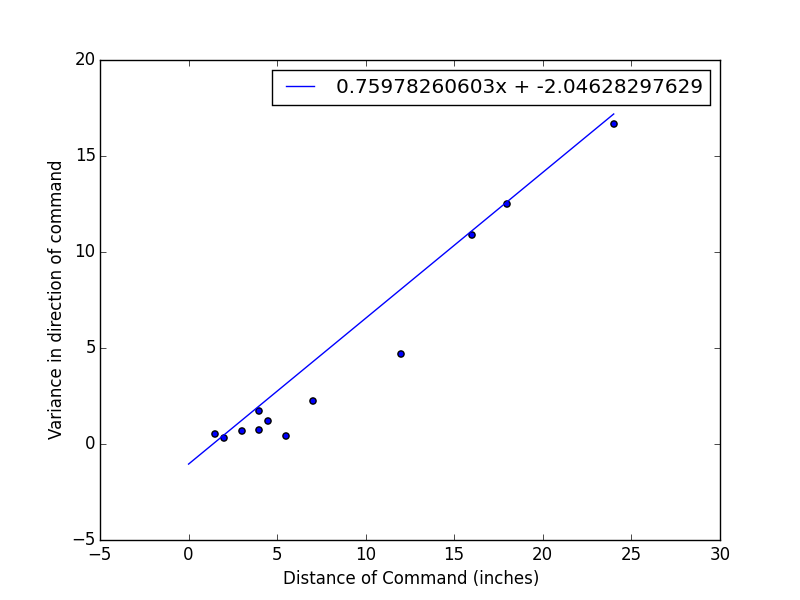
\includegraphics[scale=0.5]{images/varplot.png}
\caption{Plot of variance versus command distance}
\label{fig:varplot}
\end{figure}

To arrive at these features, we make three assumptions about the data. First, that the data are distributed in a gaussian manner. Second, that the variance in the direction of the command (i.e. in the $x$ direction for `left' or `right' and the $y$ direction for `in front' and `behind') is independent of the variance in the orthogonal direction. Third, that variance in the direction of the command scales linearly with the distance of the command, while variance in the orthogonal direction is constant. \\
\\
From this, our goal is to generate features that tell us about the probability of a point $(x, y)$ given $\lambda, \Gamma$. Let $v = (x, y) - \hat{\mu}$. A gaussian version of this probability incorporating the above assumptions would be:
\[
\frac{1}{Z}\exp\bigg(\frac{\langle v, \lambda_r\rangle^2}{k_1 \lambda_d}\bigg)\exp\bigg(\frac{[v - \langle v, \lambda_r\rangle\lambda_r]^2}{k_2}\bigg)
\]
Turning these into features in a log-linear distribution, we then get:
\begin{equation*}
\begin{split}
T_1(x, y | \lambda, \Gamma) &= \frac{1}{\lambda_d} \langle v, \lambda_r \rangle^2 \\
T_2(x, y | \lambda, \Gamma) &= [v - \langle v, \lambda_r \rangle\lambda_r]^2 \\
\end{split}
\end{equation*}
with $v = (x, y) - \hat{\mu}$ as before.

\subsection*{Calculating $T_3$}
$T_3$ is a hinge loss, designed to penalize points that are closer to an object other than the reference object (the one used in the command). The value should be zero for points where the reference object is the closest object, and increase linearly as $(x, y)$ get closer to some other object. Let $p_{(x, y), \gamma_i}$ be the point on $\gamma_i$ closest to $(x, y)$. Then,
\[
T_3(x, y|\lambda, \Gamma) = ||(x, y) - p_{(x, y), \gamma_{\refobj}}|| - \min_{\gamma_i \in \Gamma} ||(x, y) - p_{(x, y), \gamma_i}||
\]

\subsection*{Calculating $T_4$}
$T_4$ is a hinge loss, designed to penalize points that are closer to a wall than to the reference object. The value should be zero for points where the reference object is closer than any wall, and increase linearly as $(x, y)$ get closer to some other object. Let $p_{(x, y), \gamma_i}$ be the point on $\gamma_i$ closest to $(x, y)$. Then,
\[
T_4(x, y|\lambda, \Gamma) = \max\Big(0, ||(x, y) - p_{(x, y), \gamma_{\refobj}}|| - \min_{\gamma_{\textmd{wall}_i} \in \Gamma} ||(x, y) - p_{(x, y), \gamma_{\textmd{wall}_i}}||\Big)
\]

\section*{Putting the Model Together}
All the features described above are related to each other via the following graphical model:\indent\vspace{-10pt}
\begin{center}
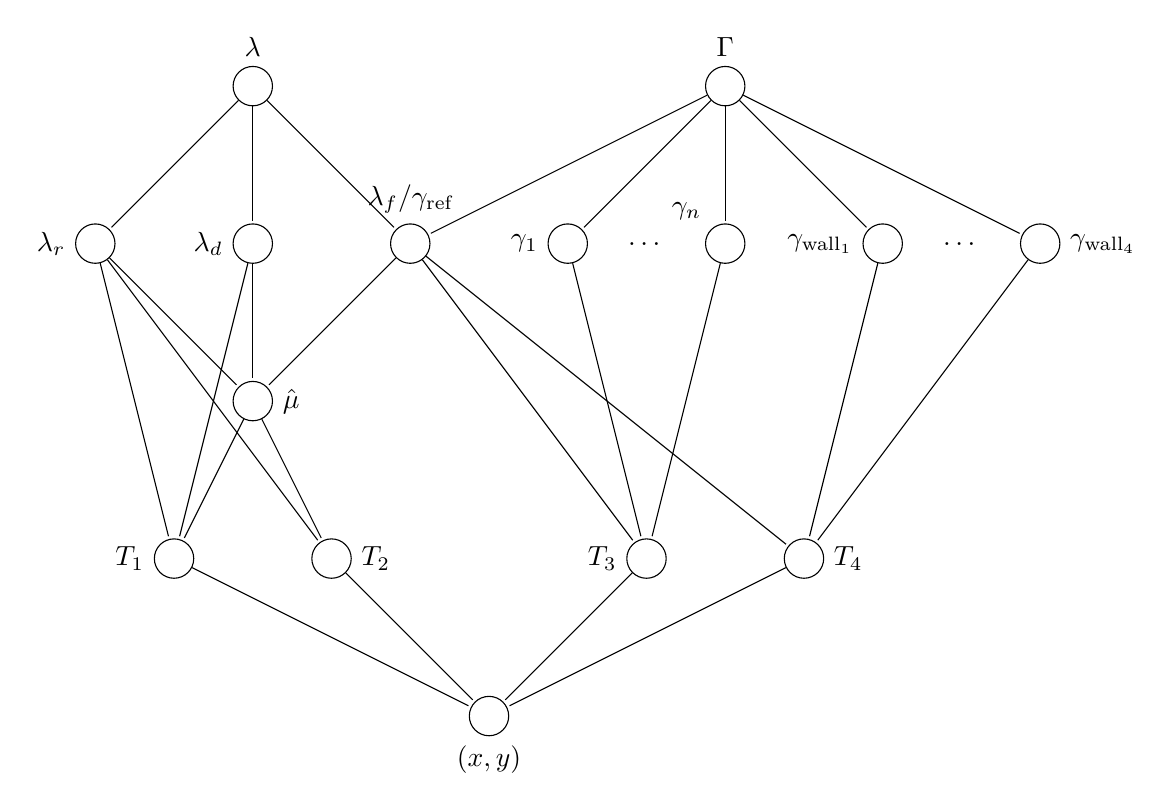
\begin{tikzpicture}[-, >=stealth', shorten >=1pt, auto, node distance=2cm, every state/.style={fill=white, draw=black, text=black, minimum size=0.5cm}]
	\node[state, label=above:$\lambda$] (cmd) {};
	\node[state, label=above:$\Gamma$] (world) [right of=cmd, xshift=4cm] {};
	\node[state, label=left:$\lambda_d$] (dist) [below of=cmd] {};
	\node[state, label=left:$\lambda_r$] (dir) [left of=dist] {};
	\node[state, label=above:$\lambda_f/\gamma_{\refobj}$] (ref) [right of=dist] {};
	\node[state, label=left:$\gamma_1$] (obj1) [below of=world, xshift=-2cm] {};
	\node[state, label=above left:$\gamma_n$] (objn) [right of=obj1] {};
	\node[state, label=left:$\gamma_{\textmd{wall}_1}$] (wall1) [right of=objn] {};
	\node[state, label=right:$\gamma_{\textmd{wall}_4}$] (wall4) [right of=wall1] {};
	\node[state, label=right:$\hat{\mu}$] (mu) [below of=dist] {};
	\node[state, label=left:$T_1$] (t1) [below of=mu, xshift=-1cm] {};
	\node[state, label=right:$T_2$] (t2) [right of=t1] {};
	\node[state, label=left:$T_3$] (t3) [right of=t2, xshift=2cm] {};
	\node[state, label=right:$T_4$] (t4) [right of=t3] {};
	\node[state, label=below:${(x, y)}$] (pt) [below of=t2, xshift=2cm] {};
	
	\path (cmd) edge (dist)
	         (cmd) edge (dir)
	         (cmd) edge (ref)
	         (world) edge (ref)
	         (world) edge (obj1)
	         (world) edge (objn)
	         (world) edge (wall1)
	         (world) edge (wall4)
	         (obj1) -- node[auto=false]{\ldots} (objn)
	         (wall1) -- node[auto=false]{\ldots} (wall4)
	         (dir) edge (mu)
	         (dist) edge (mu)
	         (ref) edge (mu)
	         (dir) edge (t1)
	         (dir) edge (t2)
	         (dist) edge (t1)
	         (mu) edge (t1)
	         (mu) edge (t2)
	         (ref) edge (t3)
	         (ref) edge (t4)
	         (obj1) edge (t3)
	         (objn) edge (t3)
	         (wall1) edge (t4)
	         (wall4) edge (t4)
	         (t1) edge (pt)
	         (t2) edge (pt)
	         (t3) edge (pt)
	         (t4) edge (pt);


\end{tikzpicture}
\end{center}

Given these features, we obtain the log-linear model
\[
\mathbb{P}_w(x, y|\lambda, \Gamma) = \frac{1}{z_w(\lambda, \Gamma)}\exp\bigg(\sum_{c = 1}^4w_cT_c(x, y|\lambda, \Gamma)\bigg)
\]
where $w$ is a vector of weights. We then learn the weights using MLE estimation.

\subsection*{MLE Estimation for Learning Weights}
We trained the model using the data from scene \#1. We assume each data point is an iid sample from $\prob_w(x, y|\lambda, \Gamma)$. Let the 12 commands be specified by $\lambda^{(1)}, \ldots, \lambda^{(12)}$. For each command we collected 10 data points. Let $X$ represent all the data and let $X^{(i)}_j$ be the $j$-th data point for the $i$-th command. Then the joint probability of the data points can be expressed as

\begin{equation*}
\begin{split}
\prob_w(X|\lambda^{(1)}, \ldots, \lambda^{(12)}, \Gamma) &= \prod_{i = 1}^{12}\prod_{j = 1}^{10} \frac{1}{z_w(\lambda^{(i)}, \Gamma)}\exp\bigg(\sum_{c = 1}^4w_cT_c(X^{(i)}_j|\lambda^{(i)}, \Gamma)\bigg) \\
&= \bigg(\prod_{i = 1}^{12}\prod_{j = 1}^{10} \frac{1}{z_w(\lambda^{(i)}, \Gamma)}\bigg)\bigg(\prod_{i = 1}^{12}\prod_{j = 1}^{10}\exp\bigg(\sum_{c = 1}^4w_cT_c(X^{(i)}_j|\lambda^{(i)}, \Gamma)\bigg)\bigg) \\
&= \bigg(\prod_{i = 1}^{12}\prod_{j = 1}^{10} \frac{1}{z_w(\lambda^{(i)}, \Gamma)}\bigg)\exp\bigg(\sum_{c = 1}^4w_c\sum_{i = 1}^{12}\sum_{j = 1}^{10}T_c(X^{(i)}_j|\lambda^{(i)}, \Gamma)\bigg)
\end{split}
\end{equation*}

Our goal then is to find the argmax over $w$ of this function. This is the same as finding the argmin of the negative log, so we have
\begin{equation*}
\begin{split}
w^* &= \argmin_w -\log\prob_w(X|\lambda^{(1)}, \ldots, \lambda^{(12)}, \Gamma) \\
&= \argmin_w \sum_{i = 1}^{12}\sum_{j = 1}^{10}\log(z_w(\lambda^{(i)}, \Gamma)) - \sum_{c = 1}^4w_c\sum_{i = 1}^{12}\sum_{j = 1}^{10}T_c(X^{(i)}_j|\lambda^{(i)}, \Gamma)
\end{split}
\end{equation*}

This is the sum of exponential families, one for each $i, j$. Therefore the derivative with respect to $w_c$ of the log partition function is the expected value of the $c$-th feature. Therefore, 
\[
\frac{\partial}{\partial w_c} -\log\prob_w(X|\lambda^{(1)}, \ldots, \lambda^{(12)}, \Gamma) = \sum_{i = 1}^{12}\sum_{j = 1}^{10} \E_w[T_c(x, y|\lambda^{(i)}, \Gamma)] - \sum_{i = 1}^{12}\sum_{j = 1}^{10}T_c(X^{(i)}_j|\lambda^{(i)}, \Gamma)
\]

We use this to perform gradient descent. In order to calculate the probabilities and the partition function, we discretize the table with a grid of step size 0.1 inches. Once we do this, we have all the components necessary to calculate the gradient, and so we perform gradient descent until the gradient falls below a threshold level.

\section*{Modeling Results}

We have successfully implemented this model in MATLAB and Python, and learned values of $w$ from the training data gathered in Experiment 1. Once trained using the MLE code implemented in MATLAB, our algorithm can parse a natural language command and, combined with information about the world $\Gamma$, produce a distribution over $(x, y)$ coordinates. Plotted below are distributions generated by the log-linear model with all four features enabled:

\begin{figure}
\centering
\begin{subfigure}{.5\textwidth}
  \centering
  \centerline{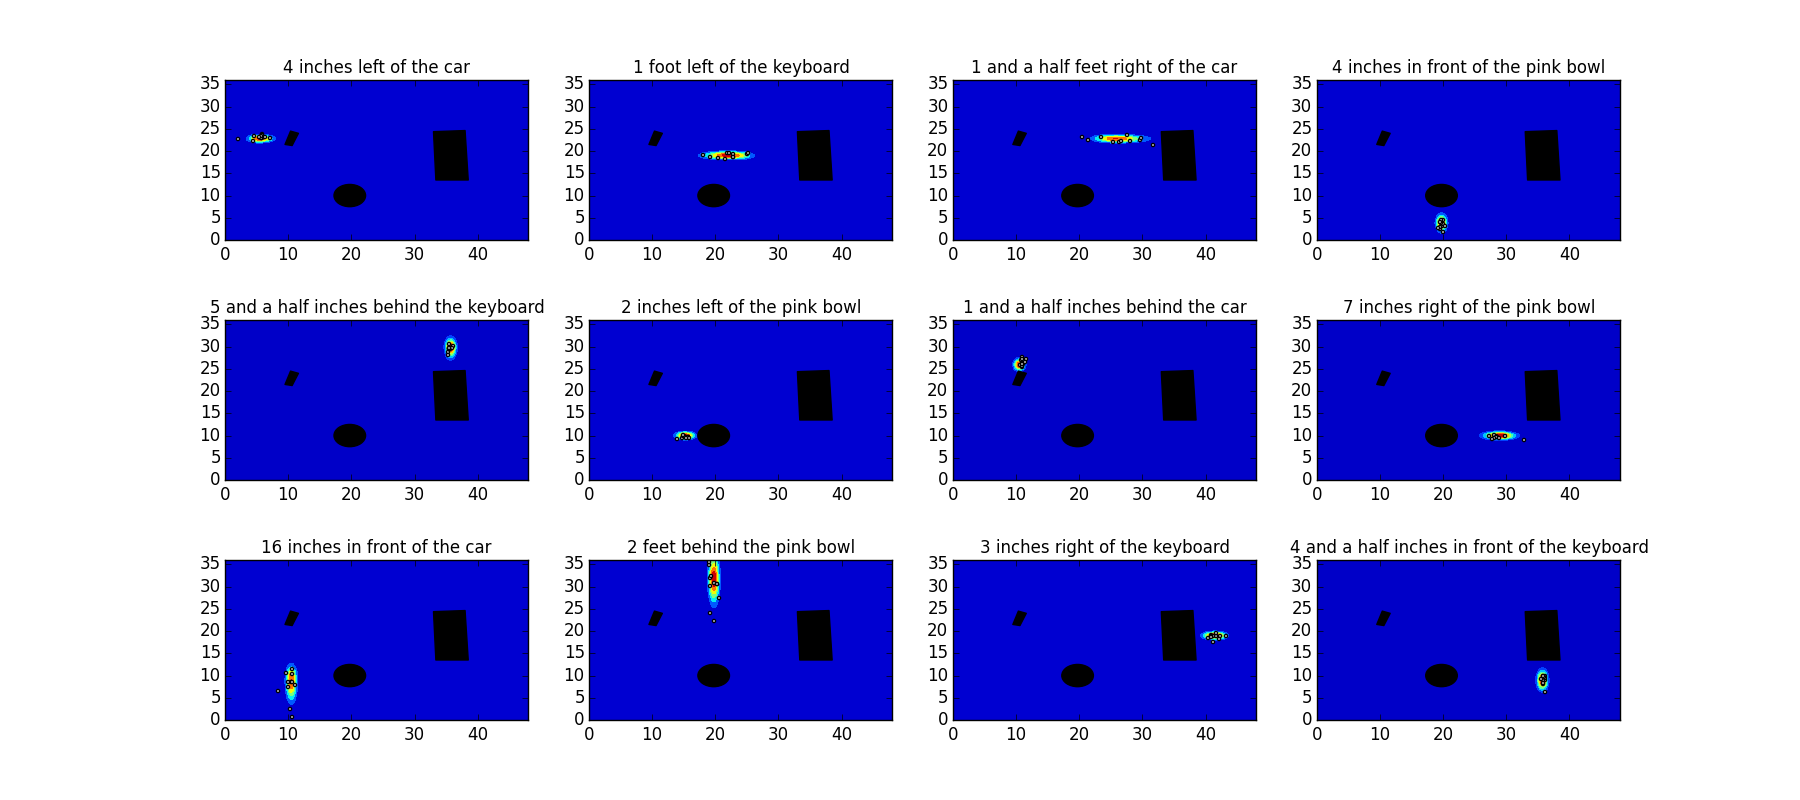
\includegraphics[scale=0.5]{images/all_commands_training.png}}
  \caption{ Distributions on training data}
  \label{fig:sub1}
\end{subfigure}
\begin{subfigure}{.5\textwidth}
  \centering
  \centerline{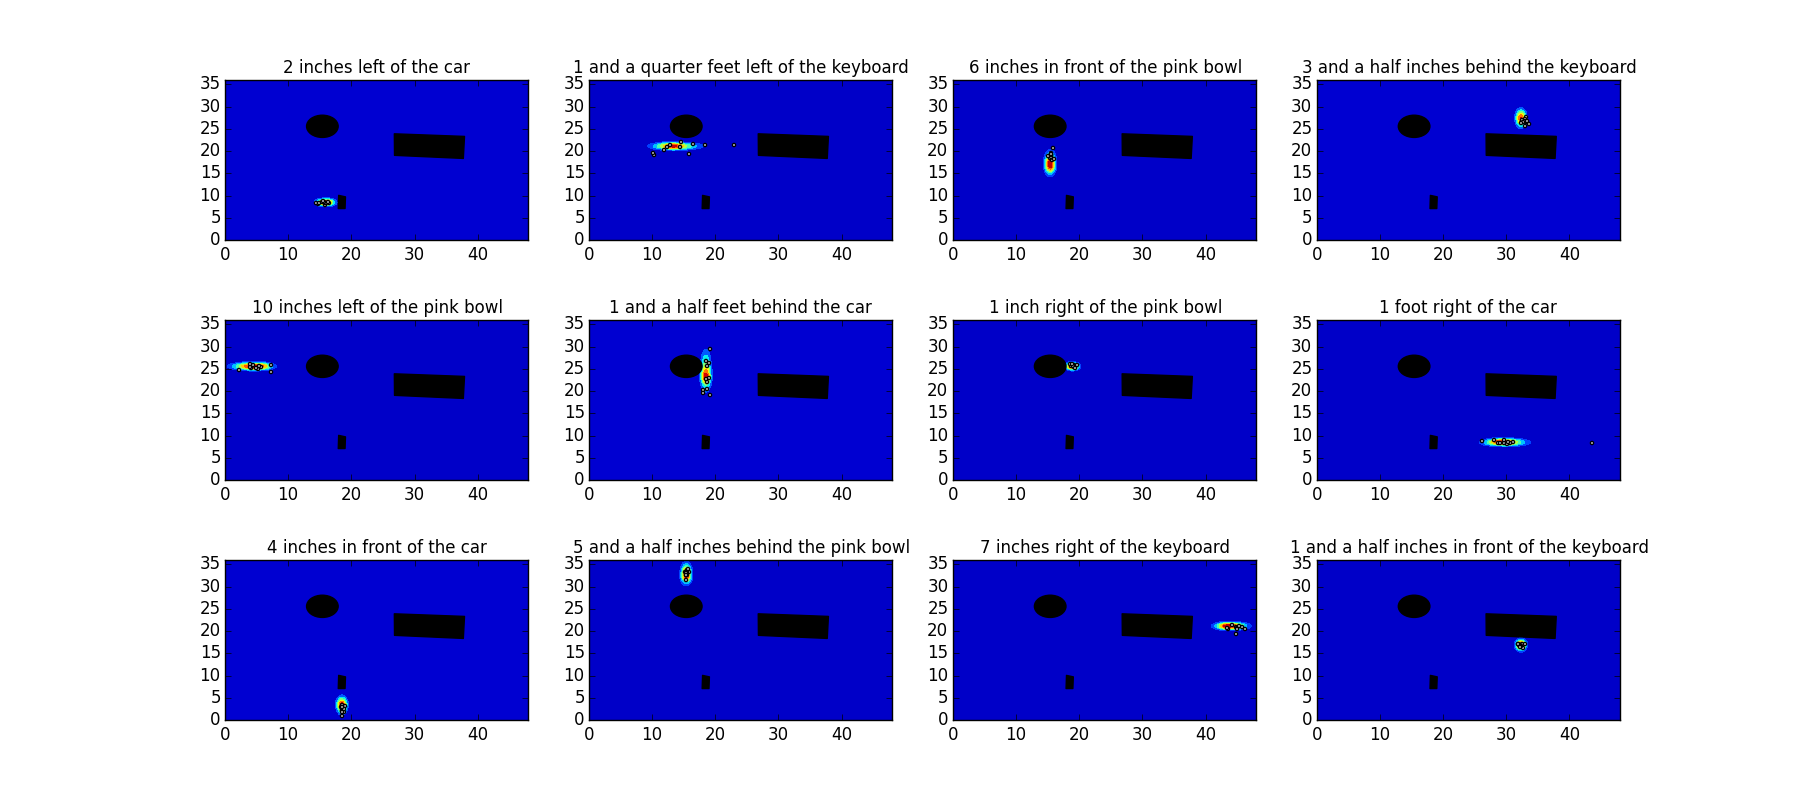
\includegraphics[scale=0.5]{images/all_commands_test.png}}
  \caption{Distributions on test data}
  \label{fig:sub2}
\end{subfigure}
\caption{Distributions from natural language commands and world information. Higher probability regions are in red.}
\label{fig:plot_distributions}
\end{figure}

\subsection*{Algorithm Evaluation}

To evaluate the performance of our algorithm, we compared its performance to a baseline algorithm that fits a gaussian distribution around $\hat{\mu}$, the naive mean generated above. In addition, we compared it to log-linear algorithms trained and tested on subsets of our features, to determine the relative performance of different feature selections. All of these algorithms were compared to an empirical Gaussian distribution generated from the data in question - i.e. fitting a Gaussian to data for the specific $\lambda, \Gamma$ pair. In the following evaluation metrics, "empirical mean" and "empirical standard deviation" refer to the mean and standard deviation of this distribution. This is distinct from the baseline algorithm, where a Gaussian distribution is generated for a $\lambda, \Gamma$ using weights learned from the entire data set. We used three different performance metrics to evaluate our system: the distance between predicted and empirical means, and the combined log-probability of the data given our distributions, mean-squared error (MSE) of the algorithms on our data sets. Plots of these metrics are displayed below, followed by a discussion of their meaning. 

\begin{figure}[H]
\centering
\begin{subfigure}{.5\textwidth}
  \centering
  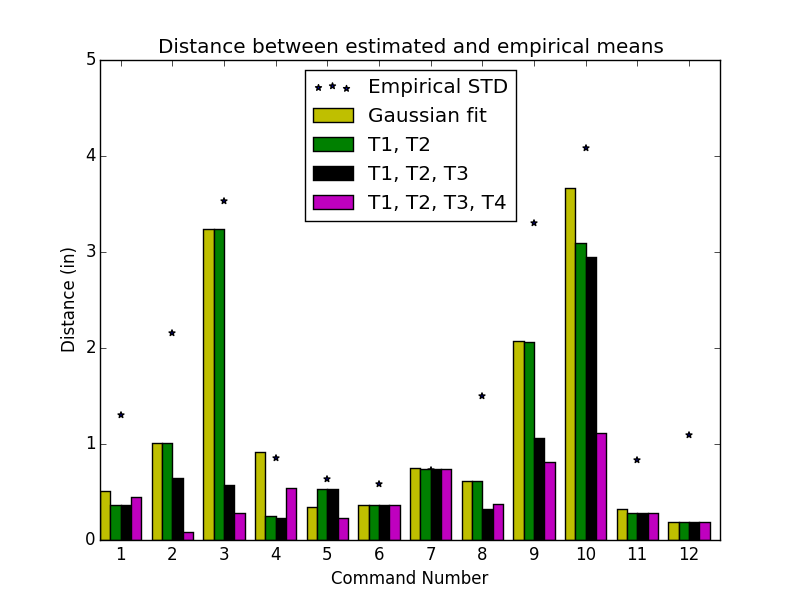
\includegraphics[width=1.1\textwidth]{images/mean_dist_training.png}
  \caption{Training data}
  \label{fig:sub1}
\end{subfigure}%
\begin{subfigure}{.5\textwidth}
  \centering
  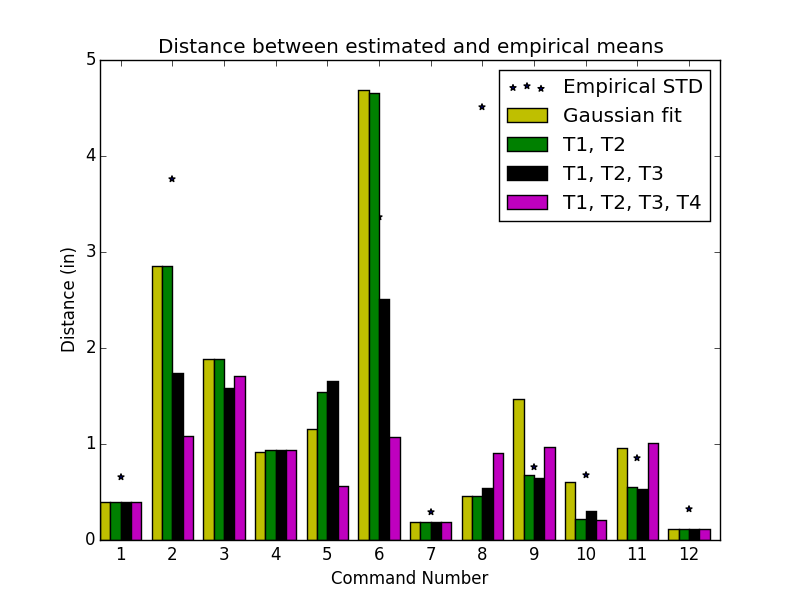
\includegraphics[width=1.1\textwidth]{images/mean_dist_test.png}
  \caption{Test data}
  \label{fig:sub2}
\end{subfigure}
\caption{Distance between empirical and predicted mean for all NL phrases. }
\label{fig:means}
\end{figure}

\begin{figure}[H]
\centering
\begin{subfigure}{.45\textwidth}
  \centering
  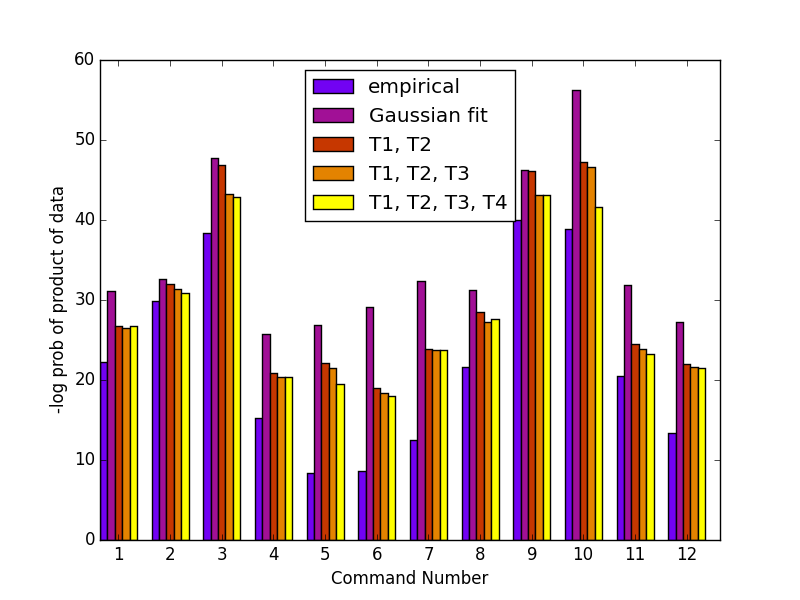
\includegraphics[width=1.1\textwidth]{images/logprob_training.png}
  \caption{Training data}
  \label{fig:sub1}
\end{subfigure}%
\begin{subfigure}{.45\textwidth}
  \centering
  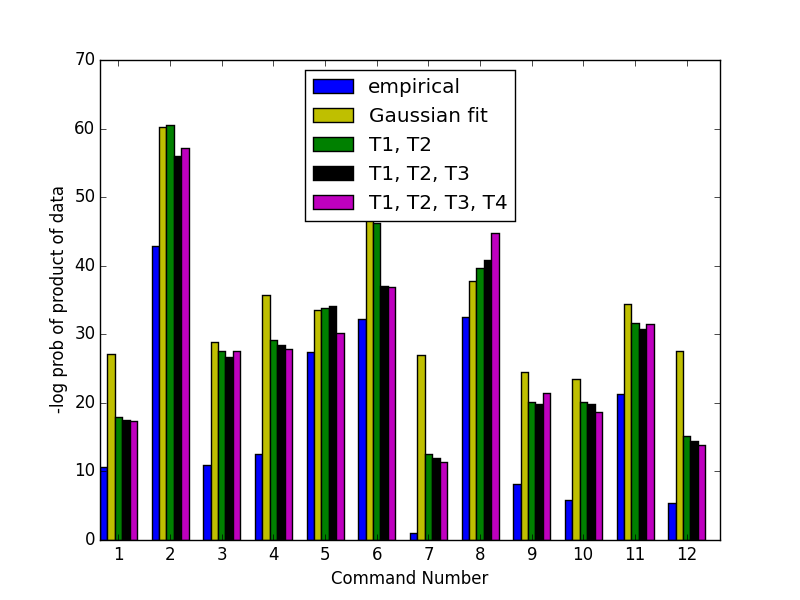
\includegraphics[width=1.1\textwidth]{images/logprob_test.png}
  \caption{Test data}
  \label{fig:sub2}
\end{subfigure}
\caption{Negative log probability of algorithms for all NL phrases}
\label{fig:logprob}
\end{figure}

\begin{figure}[H]
\centering
\begin{subfigure}{.5\textwidth}
  \centering
  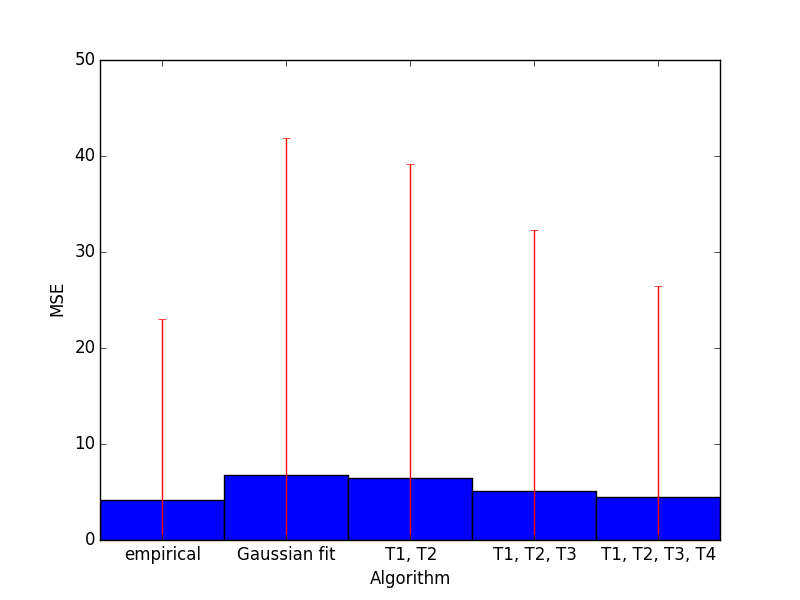
\includegraphics[width=1.1\textwidth]{images/mse_training.png}
  \caption{MSE across all training data}
  \label{fig:sub1}
\end{subfigure}% 
\begin{subfigure}{.5\textwidth}
  \centering
  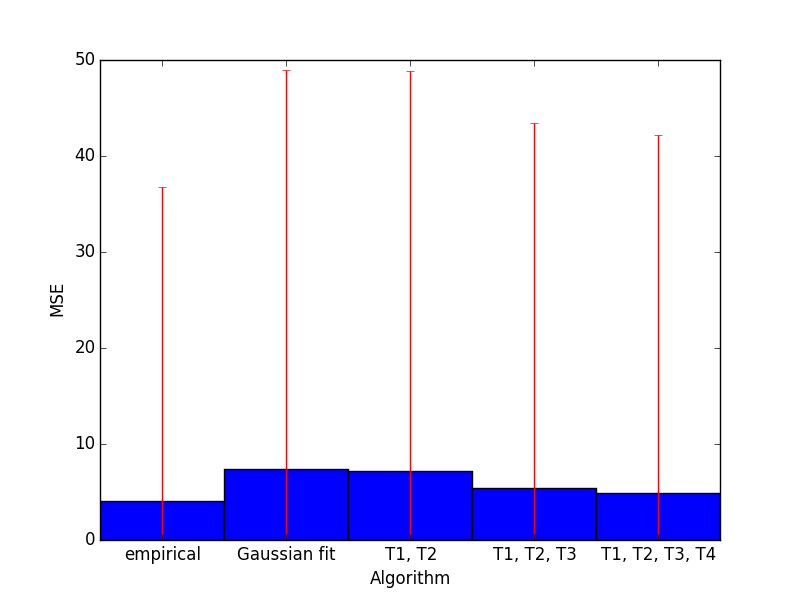
\includegraphics[width=1.1\textwidth]{images/mse_test.png}
  \caption{MSE across all test data}
  \label{fig:sub2}
\end{subfigure}
\caption{Mean-squared error by feature set. Confidence interval is twice the standard deviation of the squared error.}
\label{fig:mse}
\end{figure}

\subsection*{Discussion of Results}

These evaluation metrics lead to two primary conclusions about the performance of the algorithm and possible avenues for future research. The first, and most obvious, conclusion can be derived from the command-wise plots: the performance of different feature sets, as well as the relative performance between algorithms using different feature sets, varies across commands. This is entirely logical and consistent with the algorithms' design - in cases where objects and walls in $\Gamma$ have minimal effect, the algorithms including T3 and T4 hinge losses would be expected to perform similarly to the gaussian fit and algorithms only using the first two features. As well, in commands with short distances, the distance term in feature T1 has little effect on the variance of the distributions. However, in commands with larger distances, the non-Gaussian log-linear models have a superior performance. Overall, the larger feature sets maximize log-probability of the data, although the distance between the empirical and predicted mean varies across the commands. For nearly every command, the predicted mean is within one standard deviation of the empirical mean. A notable exception is command 4 in the test data. In that case, participants expressed confusion about reference points on the object, due to duct tape used to secure the object to the whiteboard. 

The second conclusion derives from the MSE evaluation. As shown in Figure \ref{fig:mse}, increasing the size of the feature sets lowers the mean-squared error across all distributions. However, the confidence interval with p=0.95 shows that the MSE of every feature set is statistically indistinguishable. Given that we only have 10-12 data points per $\lambda, \Gamma$ pair, a large confidence interval is to be expected. In particular, the magnitude of the standard deviation is similar to that of the empirical distribution, demonstrating that the algorithms perform similarly in that regard. Even so, the small data sets do not allow a definitive conclusion on the relative performance of each feature set. While the complete feature set does look promising in regards to log-probability, distance between predicted and empirical means, and MSE, we cannot definitively say that the performance of the log-linear model with all features is superior to Gaussian or log-linear models with smaller feature sets. Discussion of how we plan to resolve this issue, and expand the capabilities of our model, is included below.

\section*{Future Research}

\section*{Conclusion}

\end{document}